% !TeX root = ../main.tex
% Add the above to each chapter to make compiling the PDF easier in some editors.

\chapter{Approach}\label{chapter:approach}

In this research's scope, we propose a new concurrent range-locking design that leverages a probabilistic concurrent skip list~\parencite{herlihy2006provably, herlihy2020art}. It consists of two main functions:
\begin{itemize}
    \item \textbf{try\_lock}: The \texttt{try\_lock} function searches for the required range \texttt{[start, start+len)} in the skip list. If an overlapping range exists, indicating another thread is modifying that range, the requesting thread must wait and retry. If not, the range is added to the list, signaling that the range is reserved.
    \item \textbf{release\_lock}: The \texttt{release\_lock} function releases the lock by finding the address range in the skip list and removing it accordingly.
\end{itemize} 

Our range lock design also utilizes the per-node lock instead of an interval lock, thus addressing the bottleneck problem of the spinlock-based range lock and maintaining the lock's high level of performance. 

\section{Skip List}

A skip list is a probabilistic data structure that allows fast search, insertion, and deletion. It is an alternative to balanced trees, such as AVL trees or red-black trees~\parencite{pugh1990skip, pugh1990skip2}. The key idea of a skip list is to use multiple layers of sorted linked lists to maintain elements, where each layer is an "express lane" for faster traversal.

\begin{figure}[h]
    \centering
    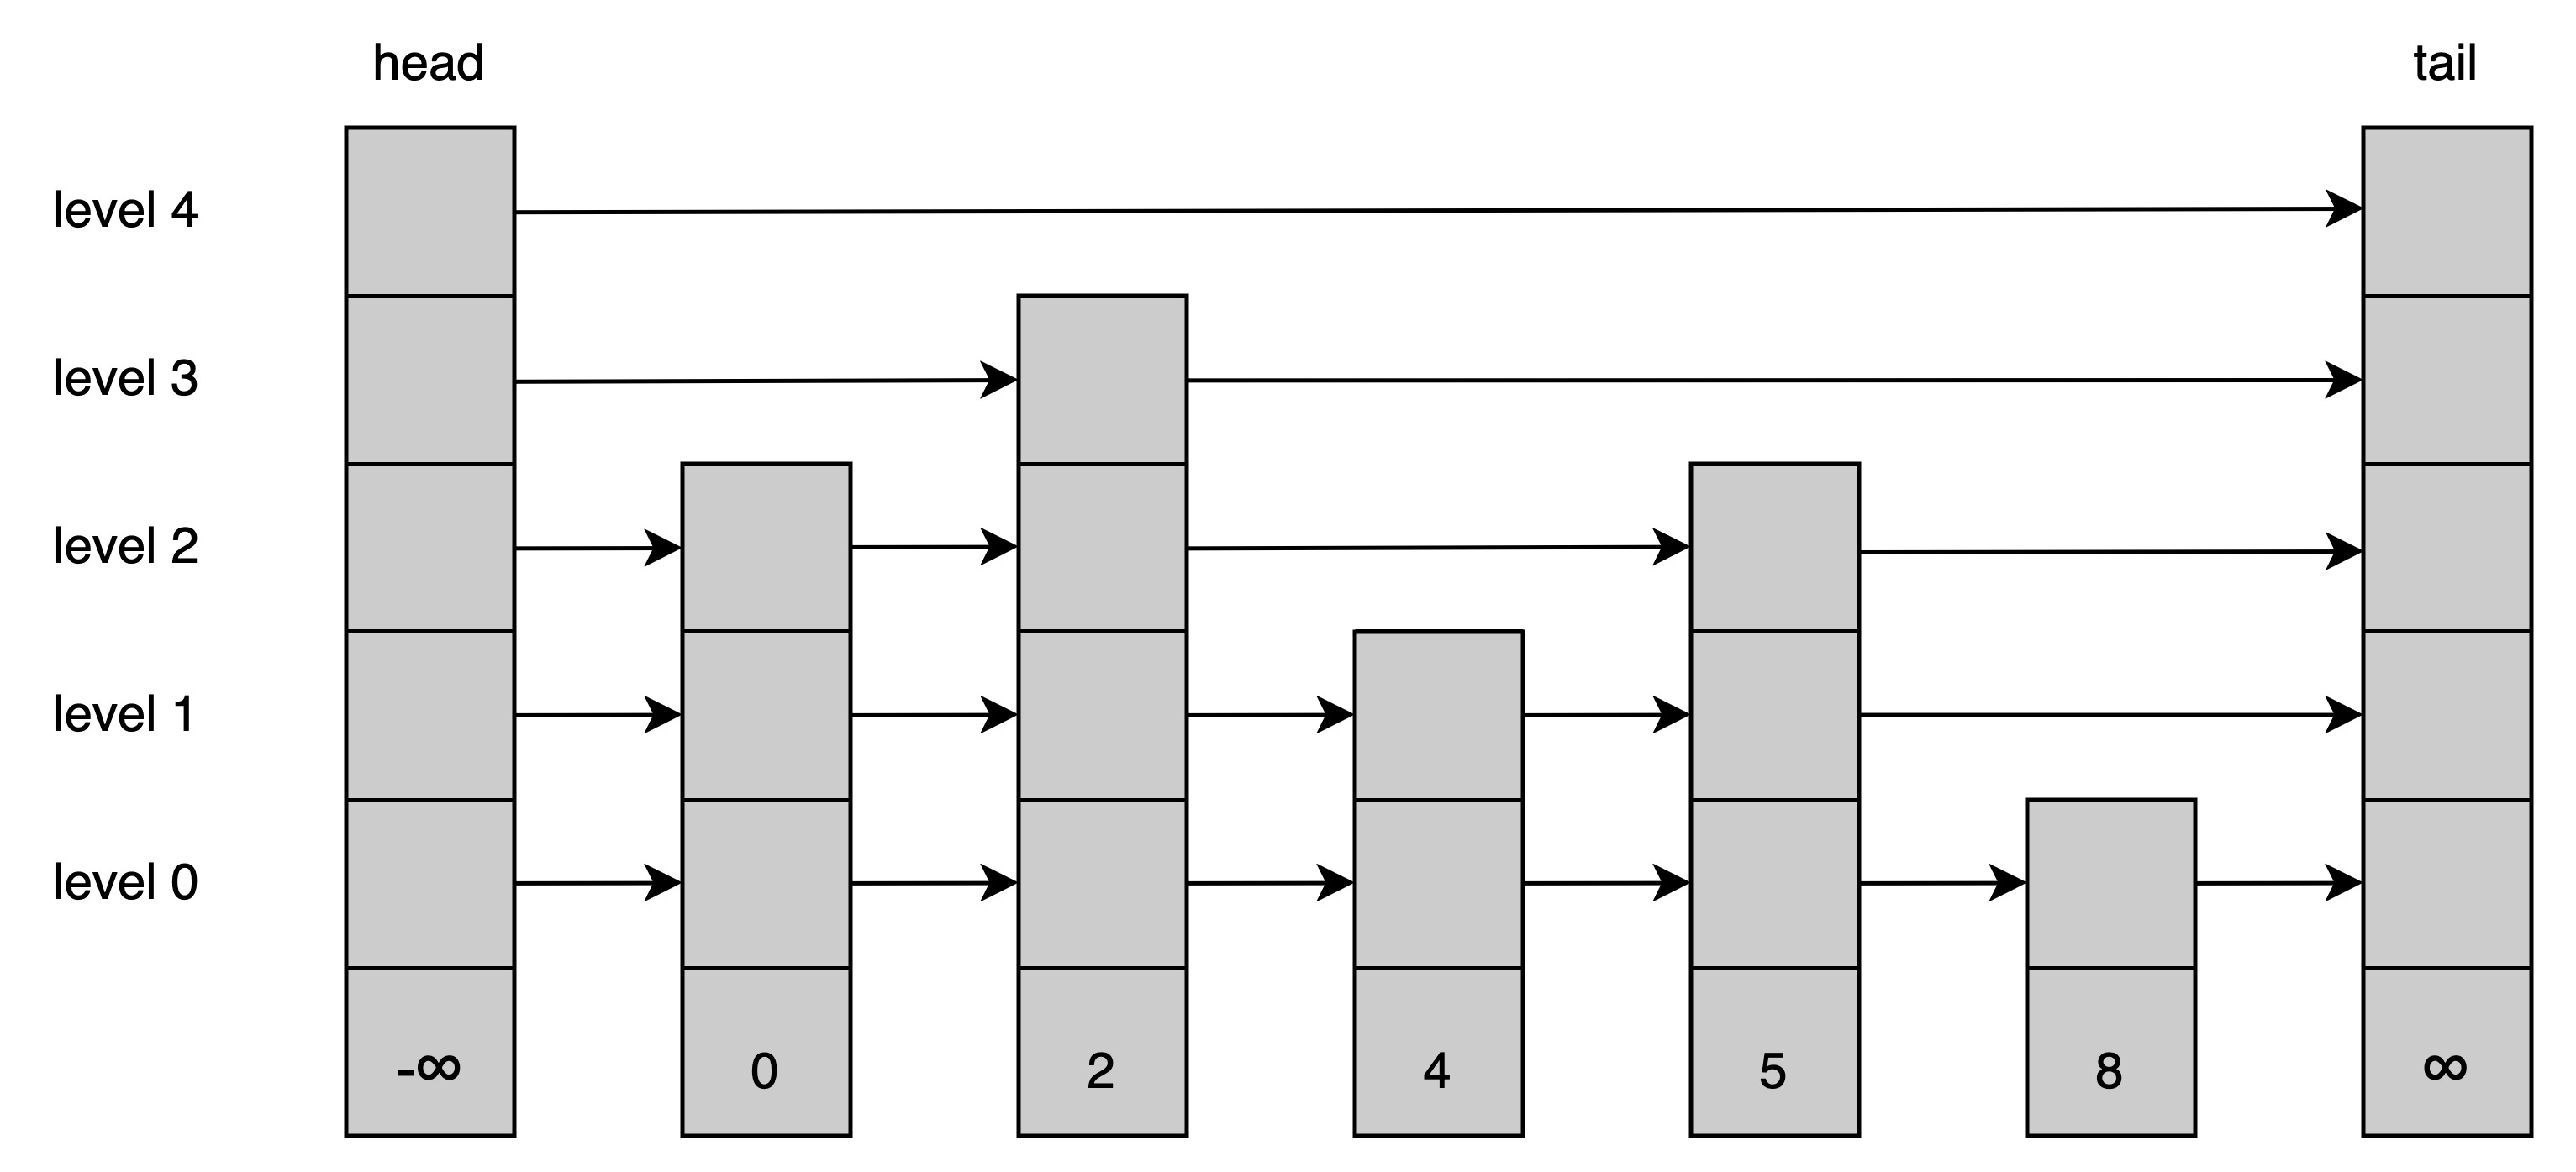
\includegraphics[width=0.8\textwidth]{./figures/skiplist.jpg}
    \caption{Skip List: this example has five levels of sorted linked lists. \\
    Each node has an unique key, and the head and tail have $-\infty$ and $+\infty$ keys.}
    \label{fig:skiplist}
\end{figure}

\subsection*{How it work}

\textbf{Layers:} A skip list consists of multiple layers. The bottom-most layer is a regular sorted linked list. Each higher layer acts as an "express lane" to speed up access by skipping over multiple elements from the layer below.

\textbf{Probabilistic Balancing:} When a new element is inserted, a node with a random height is generated. This random generation ensures that the list structure remains balanced. Consequently, skip list insertion and deletion algorithms are much simpler and faster than equivalent algorithms for balanced trees.

\textbf{Search Operation:} To search for an element, the search starts at the top-most layer and moves horizontally until it finds an element greater than or equal to the target element. If it finds an element greater than the target, it drops to the next lower layer and continues the search. This process repeats until the element is found or the search reaches the bottom-most layer without finding the target.

\textbf{Insertion and Deletion:} Inserting an element involves placing it in the appropriate position in the bottom-most layer and then possibly promoting it to higher layers based on the coin flips. Deleting an element involves removing it from all layers in which it appears.

\begin{figure}[h]
    \centering
    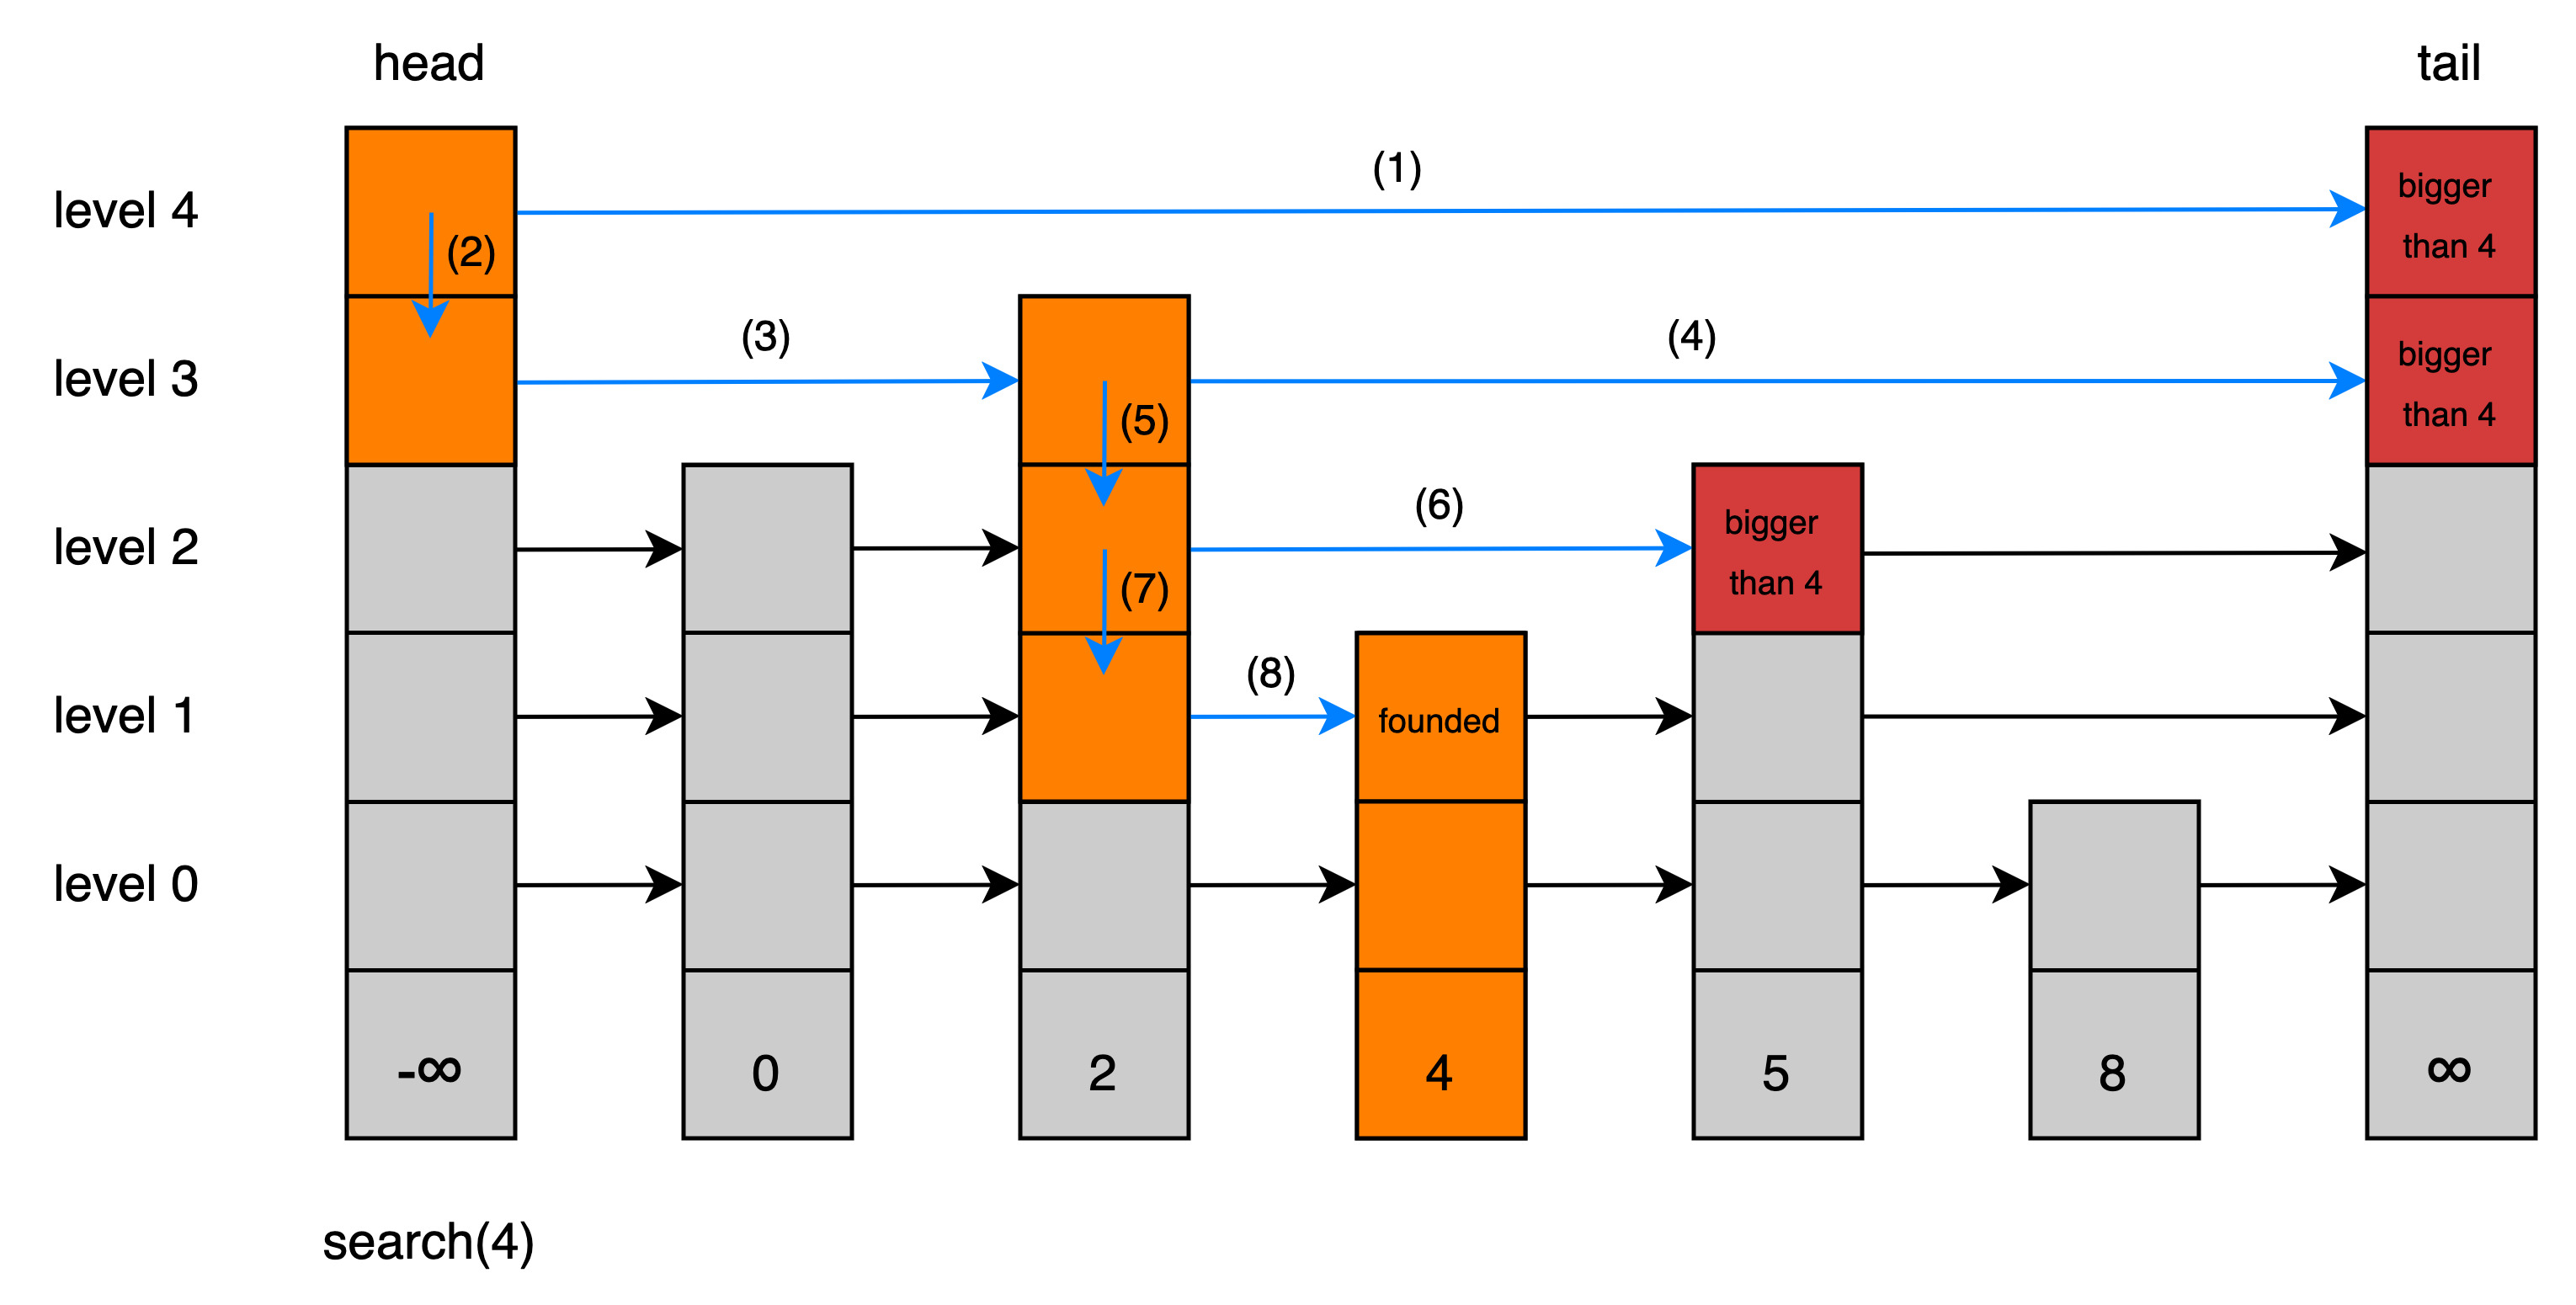
\includegraphics[width=0.8\textwidth]{./figures/skiplistsearch.jpg}
    \caption{Skip List: In this example, the list searches for a node with value 4. It starts on the head node on the highest level, tries to move horizontally until it reaches a greater value than 4, and then goes down a level and repeats. The number noted on the arrows implies the order of the traversal.}
    \label{fig:skiplistsearch}
\end{figure}

Despite their theoretically poor worst-case performance, skip lists rarely exhibit worst-case behavior, making them efficient in most scenarios. For instance, in a dictionary with over 250 elements, the likelihood of a search taking more than three times the expected duration is less than one in a million~\parencite{pugh1990skip2}. Skip lists are ideal for implementing range locks, offering a balanced structure that improves concurrency.


\begin{table}[h!]
    \centering
    \begin{tabular}{|c|c|c|c|}
        \hline
        \textbf{Operation} & \textbf{Best Case} & \textbf{Average Case} & \textbf{Worst Case} \\ \hline
 Search, Insert, Delete & $O(1)$ & $O(\log n)$ & $O(n)$ \\ \hline
    \end{tabular}
    \caption{Time complexities of skip list operations}
    \label{table:skiplisttimecomplexity}
\end{table}

\newpage

\section{Concurrent Range Lock}

We developed our concurrent range lock based on the LazySkipList technique proposed by Herlihy et al.~\parencite{herlihy2020art}. In their work, the authors introduced a LazySkipList. To summarize, the LazySkipList holds lock on all nodes to be modified, validates that nothing important has changed, completes the modifications, and releases the locks (in this context, the fullyLinked flag acts like a lock). We made some modifications to adapt this structure to our concurrent range lock.

\subsection{Node}

The structure of a node is designed to facilitate efficient concurrent operations. Each node contains several fields: \textbf\texttt{{{start}}} and \textbf{\texttt{\texttt{end}}}, which represent the aquired range associated with the node; \textbf{\texttt{{topLevel}}}, an integer indicating the highest level of the skip list in which this node appears; and \textbf{\texttt{next}}, an array of node pointers, where each element points to the next node at the corresponding level of the skip list. A node's i$^{th}$ next pointer points to the next node at level i or higher. 

Additionally, the node has two boolean flags, \textbf{\texttt{{marked}}} and \textbf{\texttt{{fullyLinked}}}. The \textbf{\texttt{{marked}}} flag indicates whether the node has been logically removed from the skip list, while the \texttt{\textbf{{fullyLinked}}} flag signifies whether the node has been fully integrated into all its intended levels in the skip list. Moreover, to ensure thread safety during concurrent operations, each node includes a recursive mutex  to control access. 

The node's methods include a constructor  for initialization, a destructor for cleanup, and lock and unlock methods to manage the mutex. There are also methods to retrieve the node's topLevel, start, and end values, ensuring that the node's properties can be accessed and modified safely in a multi-threaded environment. This structure supports the node's participation in multiple levels of the skip list, enabling efficient and safe concurrent modifications.

\begin{lstlisting}[language=C++, caption=Node structure]
    struct Node {
        Node **next;
        bool marked = false; 
        bool fullyLinked = false;

      private:
        T start; T end;
        int topLevel;
        mutable std::recursive_mutex mutex;
    };

    Node<T>::Node(T start, T end, int level) : start{start}, end{end}, topLevel{level} {
        next = new Node<T>*[level + 1];
    }

    void Node<T>::lock() { mutex.lock(); }

    void Node<T>::unlock() { mutex.unlock(); }

    int Node<T>::getTopLevel() const { return topLevel; }

    T Node<T>::getStart() const { return start; }

    T Node<T>::getEnd() const { return end; }
\end{lstlisting}